\chapter{Lunedì 01/03/2021}
\section{Scopo del corso}
\paragraph{Catena} Il corso è parte di una catena che inizia con Reti logiche e finisce con Sistemi operativi, un percorso che va dal calcolatore al sistema operativo.
\paragraph{Argomenti principali} Il corso completa la spiegazione della parte hardware di un calcolatore (iniziata con Reti logiche) introducendo i seguenti argomenti:
\begin{itemize}
	\item interruzioni;
	\item protezioni;
	\item memoria virtuale (paginazione).
\end{itemize}
queste cose ci permetteranno di implementare la cosiddetta \textbf{multiprogrammazione}, ossia la capacità di eseguire più di un programma alla volta. Questa cosa, attenzione, non dipende dalla presenza di più di un processore (in questo corso non parleremo di multiprocessore).
\paragraph{Nucleo di un sistema operativo} Come da tradizione non ci limiteremo a queste cose chiaccherando: realizzeremo un nucleo di sistema operativo in grado di eseguire più programmi in contemporanea.

\section{La confusione iniziale} 
Il fatto che noi studiamo la struttura del calcolatore avendo già avuto a che fare con un sistema operativo è un problema. Le numerose modifiche apportate ai calcolatori per renderli più efficienti hanno portato ad avere uno strato di software molto spesso: ciò nasconde ai nostri occhi ciò che realmente avviene in un calcolatore, quindi ci porta a pensare cavolate.
\paragraph{Domanda da ripetersi ogni volta} \underline{\underline{Chi}} fa cosa? Dobbiamo essere in grado di dire, in qualunque situazione, chi fa una certa cosa all'interno di un calcolatore. In un contesto ad elevata astrazione è facile dire, \emph{di fronte a una scena del crimine}, \emph{che il colpevole è il coltello}.
\paragraph{Le tre divinità} In questa nuvola di incertezza e ignoranza siamo abituati a sopravvalutare il potere delle varie componenti di un calcolatore. Noi abbiamo tre divinità:
\begin{itemize}
	\item processore
	\item sistema operativo (il software)
	\item compilatore (l'angelo custode dei nostri programmi)
\end{itemize}
in questo corso lo scopo è \textbf{uccidere} queste tre divinità, cioè rendere chiaro cosa effettivamente fanno queste componenti.

\section{Facciamo un passo indietro: il Manchester Baby}
\paragraph{Soluzione} Per eliminare la confusione iniziale cosa buona è tornare indietro nel tempo e ripartire dalle cose semplici.
\paragraph{Manchester Baby} Il calcolatore SSEM (\emph{Small-Scale Experimental Machine}), detto \emph{Manchester Baby}, è stato realizzato nel 1948 e può essere considerato il  "primo computer moderno" (mettere tra tante virgolette). Perché diciamo questo?
\begin{itemize}
	\item Presenta un concetto importante tipico dei calcolatori moderni: la centralità della memoria (e non del processore).
	\item La memoria di cui parliamo, implementata con un tubo catodico, è organizzata in celle: ogni cella ha un numero (un valore) ed è identificata da un indirizzo.
	\item Risulta possibile accedere liberamente a queste celle, in qualunque ordine (accedere significa leggere o scrivere nella cella).
\end{itemize}
Gli indirizzi sono una delle cose più nascoste dal lato software, ma anche una delle cose più importanti da comprendere per analizzare il comportamento di un calcolatore (l'idea base dell'architettura è quella di una via piena di case, ciascuna con un numero civico, che possiamo visitare per conoscerne i proprietari o per sostituirli). 
\paragraph{Andiamo ancora indietro} Questo tipo di memoria è stato pensato anche nell'800, ma l'idea era utilizzare la memoria esclusivamente per i dati.
\paragraph{Quindi} La novità più rivoluzionaria è l'uso della memoria per ospitare non solo i dati da elaborare, ma ANCHE le istruzioni da eseguire  (il programma).
\paragraph{Lo scopo iniziale del calcolatore e le conseguenti evoluzioni} I calcolatori sono stati pensati dai pionieri per eseguire operazioni aritmetiche (\emph{calcolatori} nel senso di \emph{calcolare}), dunque gli schemi pensati sono stati calati forzatamente in altre situazioni. Pensiamo alla MOV: si eredita il concetto degli \emph{operandi} (ripensare all'istruzione in Assembler, definiamo i parametri di ingresso col nome di operandi).

\paragraph{Input e Output} L'unica forma di ingresso è caratterizzata da un pannello: abbiamo delle file di bottoni che permettono di settare i bit, singolarmente (si hanno almeno 32 bottoni). Prima seleziono (attraverso altri bottoni) la riga, dopo setto i bit che mi interessano.
\begin{center}
	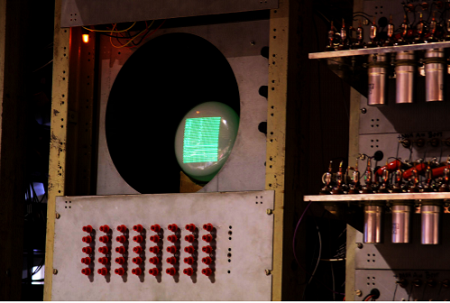
\includegraphics{img/3.PNG}
\end{center}
Il Manchester Baby fu costruito per testare una nuova tecnologia (nuova nel 1948) basata sui tubi catodici: i bit sono memorizzati come punti o linee su uno schermo fluorescente, vengono scritti dirigendo opportunamente un raggio catodico e riletti tramite una griglia metallica che copre lo schermo. Il vantaggio di avere una memoria a tubo catodico è la possibilità di vederne un'immagine rappresentativa con un normale schermo a tubo catodico (come quello dei vecchi televisori). Si osservi una cosa: il software non ha controllo dell'I/O, differenza sostanziale rispetto ad oggi.

\paragraph{Caratteristiche della memoria e registri}
\begin{center}
	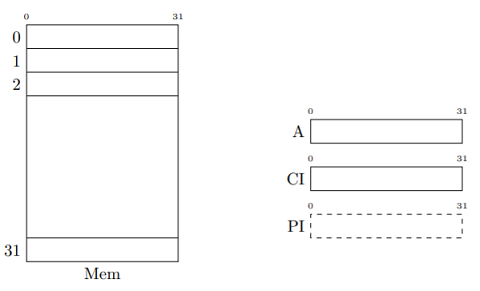
\includegraphics{img/4.PNG}
\end{center}
\begin{itemize}
	\item Abbiamo celle di dimensione a 32 bit. 
	\item Contrariamente a quanto già visto la cifra più significativa sta in posizione 0 e non nell'ultima posizione della cella (ne dobbiamo tenere conto).
	\item Gli indirizzi non sono visibili sullo schermo, ma posti in input con i bottoni del Manchester Baby, Si impostano i bottoni per ottenere una particolare riga e a quel punto la si manipola.
\end{itemize}
Il processore del Manchester Baby presenta tre registri, tutti a 32 bit:
\begin{itemize}
	\item il registro accumulatore A
	\item il registro CI (\emph{Current Instruction})
	\item il registro PI (\emph{Present Instruction})
\end{itemize}

\paragraph{Esecuzione di istruzioni in sequenza} Il processore è una macchina che esegue istruzioni elementari contenute in memoria. Riceve dei numeri e li interpreta come istruzioni, precisamente:
\begin{enumerate}
	\item incrementa CI di 1;
	\item legge dalla memoria la locazione di indirizzo CI e la copia in PI;
	\item esegue l'istruzione contenuta in PI;
	\item se l'istruzione non era di stop, torna al punto 1; altrimenti, accende la lampadina e non fa altro.
\end{enumerate}
Questo ovviamente tenendo conto di eventuali istruzioni di salto (che modifica il contenuto di CI prima che questo venga copiato in PI). Si tenga conto che se l'indirizzo al reset di CI è zero allora la prima istruzione eseguita sarà quella posta all'indirizzo 1. Al di la di queste cose il ragionamento pensato per eseguire istruzioni in sequenza (ed effettuare eventuali salti) è praticamente uguale a quello del processore moderno.

\paragraph{Programmare} Programmare significa porre il contenuto iniziale in memoria in modo tale che la macchina possa lavorare da sola. La cosa non è cambiata: anche oggi programmare significa questo! Il numero posto in una cella, abbiamo già detto, viene considerato dal processore come un'istruzione. Vediamo formato e possibili istruzioni
\begin{center}
	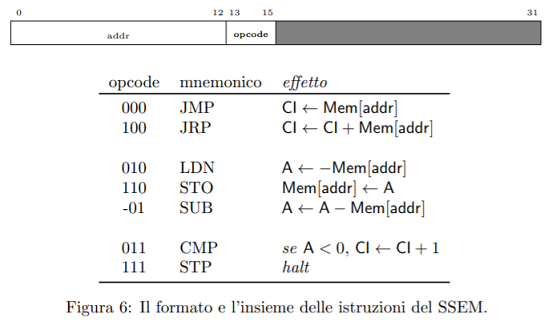
\includegraphics{img/1.PNG}
\end{center}
\begin{itemize}
	\item Formato:
	\begin{itemize}
		\item Dalla posizione 0 alla posizione 12 abbiamo l'indirizzo (\emph{addr}), cioè l'operando.
		\item Dalla posizione 13 alla posizione 15 abbiamo l'OPCODE, cioè l'identificativo dell'istruzione.
		\item I bit rimanenti non presentano contenuto rilevante.
	\end{itemize}
	\item Istruzioni:
	\begin{itemize}
		\item JMP: istruzione di salto non condizionato, pongo in CI il contenuto della cella di memoria Mem[addr]
		\item JRP: jump relativa, aggiorno CI sommando ad esso il contenuto della cella di memoria Mem[addr]
		\item LDN (\emph{LoaD Negative}: aggiorno il registro accumulatore ponendo l'opposto del numero memorizzato in Mem[addr] (rappresentazione in C2)
		\item STO: pongo come contenuto della cella di memoria Mem[addr] il contenuto del registro A.
		\item SUB: sottrazione, sottraggo al contenuto del registro A il contenuto della cella di memoria Mem[addr]. Il risultato della sottrazione è posto nel registro A. Dovendo ridurre all'osso hanno pensato che la sottrazione sia più utile (e che si possa fare un addizione utilizzando la LDN). Per fare l'addizione dobbiamo fare il seguente calcolo
		\[\text{ADDIZIONE }=-(-X-Y)\]
		\item CMP: salto condizionato, se il contenuto del registro accumulatore è minore di 0 viene saltata una istruzione (riduzione all'osso del meccanismo visto in Assembler).
		\item HLT: \emph{halt}, l'esecuzione sequenziale di istruzioni viene fermata e la spia rossa del calcolatore accesa.
	\end{itemize}
\end{itemize}
\paragraph{Esempio di programma che restituisce l'opposto}
\begin{center}
	
\includegraphics{img/2.PNG}
\end{center}
\paragraph{Ulteriore esempio} Nelle appendici è presente la dispensa di Lettieri sul Manchester Baby. Troverete un ulteriore esempio di programmazione col Manchester Baby.
\clearpage
\section{Domanda finale della lezione}
\paragraph{Chi comanda?}
\begin{itemize}
	\item La memoria è una risposta troppo generica.
	\item Il processore non può essere perché esegue gli ordini del software e sa solo ciò che è contenuto nei registri. Non conosce il programma passato, ne tantomeno quello futuro. Non conosce gli effetti complessivi di una set di istruzioni, le esegue singolarmente senza analizzarle da un punto di vista globale.
\end{itemize}
Nel calcolatore chi comanda è il software, è li che risiede l'intelligenza del programma: noi poniamo codice nella memoria, e ciascuna riga indica un'istruzione da eseguire. Questa cosa è l'essenza del \emph{calcolatore programmabile}:  \textbf{modificare ciò che il calcolatore fa senza modificare l'hardware}.
\paragraph{Flusso di controllo} Il software controlla il processore e gli fornisce l'istruzione successiva (e lo fa in modo esplicito nel caso in cui voglia compiere un'istruzione di salto). Con un processore si ha un unico flusso di controllo.
\paragraph{Cosa succede se  il software è composto da più parti?} Supponiamo di avere funzioni di libreria: cosa succede? Si dice che il programma cede il controllo del processore alla funzione di libreria (il processore è come una palla che può rimbalzare da una persona a un'altra). Alla fine la funzione di libreria restituirà il controllo al programma.